\documentclass[norsk]{beamer}
\usepackage[utf8]{inputenc}
\usepackage{listings}
\usepackage{color}
\usepackage[norsk]{babel}
\usepackage{fontspec}


\definecolor{pblue}{rgb}{0.2,0.2,0.7}
% \definecolor{pgreen}{rgb}{0,0.5,0}
\definecolor{pred}{rgb}{0.7,0.2,0.2}
\definecolor{pgrey}{rgb}{0.46,0.45,0.48}

\lstset{
	language=Python,
	numbers=left,
	breaklines=true,
	tabsize=4,
	commentstyle=\color{pgrey},
	keywordstyle=\color{pblue},
	stringstyle=\color{pred},
    showstringspaces=false,
	literate={\ \ }{{\ }}1
}

%Information to be included in the title page:
\title{Big O notation}
\author{Jakob Hansen \\ \texttt{jakobkha@uio.no}}
\date{\today}

\begin{document}
	\frame{\titlepage}

    \begin{frame}[fragile]
        \frametitle{Big O notasjon}
        \begin{itemize}
            \item Hva er målet med Big O?
            \pause
        \item Analysere kjøretid! Hvilken algoritme er raskest? (Grovt)
        \pause
        \item Abstrahere bort de små forskjellene
        \pause
        \begin{lstlisting}[basicstyle=\scriptsize]
def numExists(array : list[int], numToFind : int) -> bool:

    # Itererer over array, hvis vi finner tallet, true
    for i in range(len(array)):
        if array[i] == numToFind:
            return true

    # Ingen elementer er lik tallet, false
    return false
		\end{lstlisting}
        \end{itemize}

    \end{frame}

    \begin{frame}
        \frametitle{Big O notasjon}
        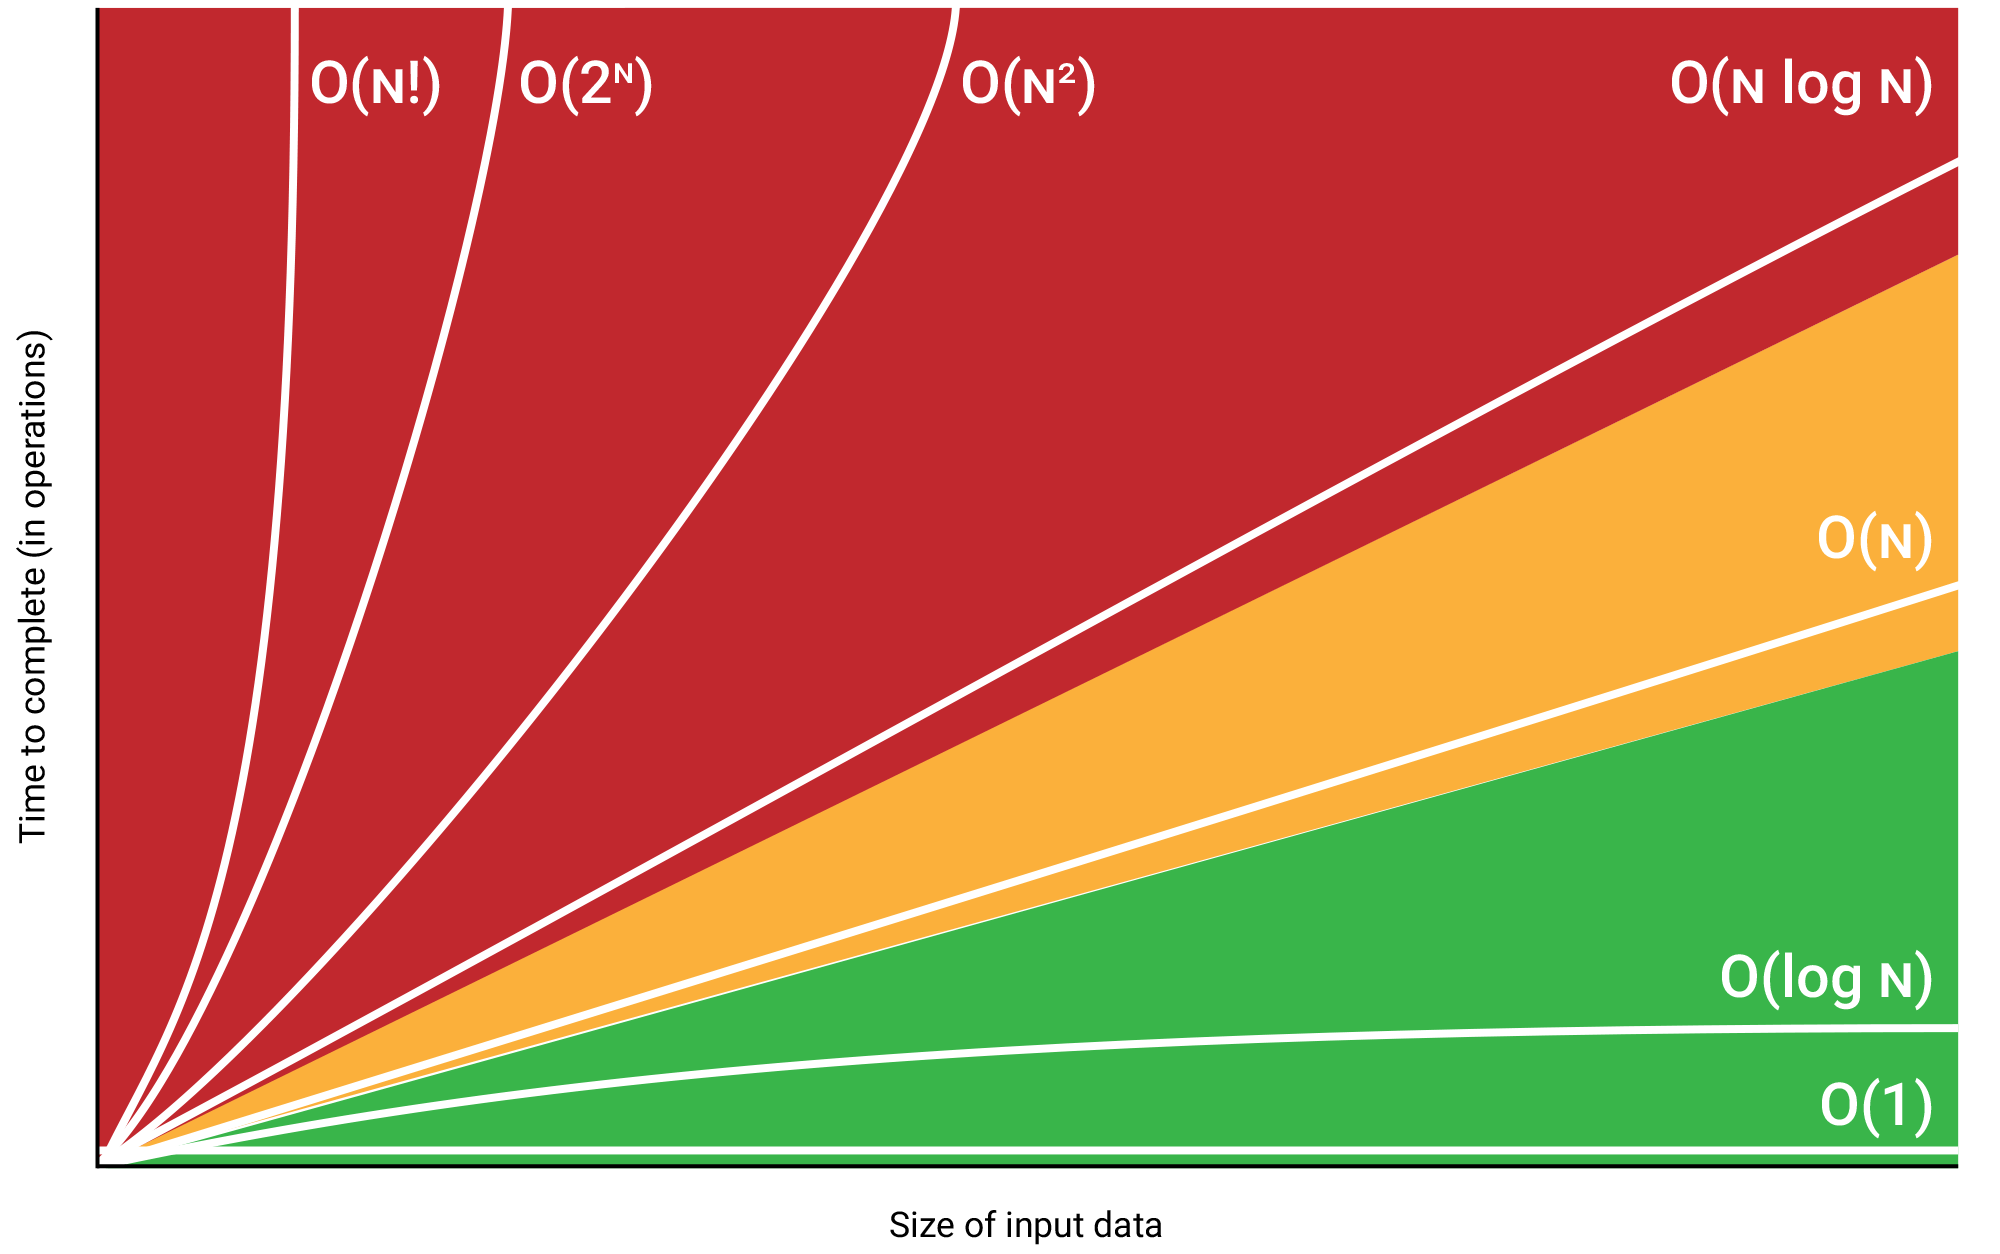
\includegraphics[keepaspectratio, width=300pt, height=300pt]{big-o-chart.png}
    \end{frame}

    \begin{frame}
        \frametitle{Konstant tid}
        \begin{itemize}
            \item O(1)
            \item Tar samme tid uansett
            \item Eksempel: Hente første element av et array
            \item O(1000) = O(1)
        \end{itemize}
    \end{frame}

    \begin{frame}
        \frametitle{Lineær tid}

        \begin{itemize}
            \item O(n)
            \item Vokser direkte med input størrelse
            \item Eksempel: Iterere og printe ut hvert element i et array
            \item O(100n) = O(n)
        \end{itemize}

    \end{frame}

    \begin{frame}
        \frametitle{Polynomiell tid}

        \begin{itemize}
            \item For hver n, for hver n...
            \item O($n^x$), for eksempel O($n^2$)
            \item Eksempel: To løkker som sjekker om det finnes en duplikat i arrayet.
            \item Eksempel: ``Bruteforce`` en kodelås
        \end{itemize}
    \end{frame}

    \begin{frame}
        \frametitle{Logaritmisk tid}

        \begin{itemize}
            \item O(log(n))
            \item Litt tricky
            \item $log_2(n) = x$ hvis $2^x = n$
            \item Antall ganger du må halvere n for å få 1
            \item Eksempel: Lete i telefonbok, Binary search
            \item Senere: O(n log(n))
        \end{itemize}
    \end{frame}

    \begin{frame}
        \frametitle{Oppgaver!}

        \begin{center}
            \url{https://github.com/jakobkhansen/IN2010_h2021}
        \end{center}
    \end{frame}

\end{document}

